\documentclass[11pt, a4paper]{article}

\usepackage{url}
\usepackage{cite}
\usepackage{times}
\usepackage{float}
\usepackage{caption}
\usepackage{courier}
\usepackage{hyperref}
\usepackage{breakurl}
\usepackage{graphicx}
\usepackage{fancyhdr}
\usepackage{boolexpr}
\usepackage{multirow}
\usepackage{subfigure}
\usepackage{indentfirst}
\usepackage[inline]{enumitem}

% no color links
\hypersetup{
bookmarks=false,
colorlinks=true,
citecolor=black,
filecolor=black,
linkcolor=black,
urlcolor=black,
pagebackref=true
} 

% compact bibliography
\let\oldthebibliography=\thebibliography
\let\endoldthebibliography=\endthebibliography
\renewenvironment{thebibliography}[1]{	%
	\begin{oldthebibliography}{#1}	%
	\setlength{\parskip}{0ex}	%
	\setlength{\itemsep}{0.4ex}	%
  \fontsize{7.1}{8.5}
  % tweak label width for proper alignment - two digits
  \settowidth\labelwidth{\@biblabel{99}}
	\selectfont
}{\end{oldthebibliography}}

% hacks
\newcommand{\note}[1]{\noindent\textbf{\color{red}[#1]}}
\newcommand{\comment}[1]{}

\title{\Large \bf \underline{Challenge:}\\
How might we have more transparency on where our data is going in the Internet?\\}
\author{
	Petros Gkigkis\\
	\texttt{gkigkis@ics.forth.gr}\\
	\and
  	Konstantinos Kleftogiorgos\\
	\texttt{kleftog@ics.forth.gr}\\
	\and
	Anastasia Ntagianta\\
	\texttt{dagianta@csd.uoc.gr}\\
  	\and
	Eva Papadogiannaki\\
  	\texttt{epapado@ics.forth.gr}\\
	\and
	Kostas Solomos\\
	\texttt{solomos@ics.forth.gr}\\
	\and
	Nestoras Sdoukos\\
	\texttt{sdoukos@csd.uoc.gr}\\
	\and
	Antonios Tzougkarakis\\
	\texttt{tzugarak@csd.uoc.gr}\\
}
\date{}

\pagestyle{fancy}
\fancyhf{}
\rhead{}
\lhead{CS-533: Security, Privacy and Intelligence on the Internet}
\rfoot{Page \thepage}

\begin{document}

	\pagenumbering{gobble}
	\maketitle
	\newpage
	\pagenumbering{arabic}

	\section{Challenge Description}
\label{sec_a}

\subsection{What are the aspects of the challenge you already know a lot about?
What are your assumptions?}

\paragraph{Privacy}

Our aspect is not specialized  on application layer's  user's privacy,  
but we are focusing on privacy transparency on IP and Transport layers; 
specifically on  network traffic generated by the users, and  handled by the ISPs.
An Internet Service Provider logs and stores user's traffic that contains 
personal information. 
This kind of information might be used for further analysis by the ISPs or by 
third party entities such as Universities, Researchers, companies and Law enforcers.	
So, whoever is involved in this procedure should respect the user's privacy by 
applying data protection techniques, such as anonymization in those datasets.

\paragraph{Routing and storage}

Every Autonomous System has its own routing policies to forward traffic and these 
policies are mostly kept in private. ASes can have public and private peering 
agreements. These peering connections can be direct or can be through Internet 
Exchange Points. In the case of Internet Exchange Points, there are two main 
sources to extract information about peering on IXPs. The first source is the 
PeeringDB and the second one is the Packet Clearing House (PCH). 
These sources provide information about the members of each IXP and also provide
the peering policy of each AS. 

Moreover, a lot of research has been conducted to discover the AS topology map. 
CAIDA provides a variety of datasets about ASes and Internet topology. Also there 
are many well-known methodologies to discover topologies like ``DoubleTree'' algorithm 
\cite{caida}. 
These techniques can be used  to validate our results and also provide insighs 
on the routing policies.
Furthermore, big websites, like Facebook, use multiple servers in different locations 
to handle the user traffic. Content is served to users based on their location and 
also based on the load of each server in that time. So we know that our data is 
replicated in different sites (servers) and possible different countries. 

\paragraph{Surveillance}
It has been proven that NSA is doing surveillance in Internet traffic. There are
some applications and services developed to conduct this analysis on a daily 
basis at a huge amount of data. It is known that a large amount of internet 
servers are located in US and that is one major reason why internet traffic 
boomerangs through the US. Moreover, it's possible for NSA or other intelligence
agencies to access the data.

\paragraph{Ethics}
Ethically, the personal data should not be published. The extend of a user's 
wish to share private information should not interfere with another user's 
choice of data sharing.  For example, in some cases law enforcement has the 
ability to collect and use certain information when they are investigating 
crimes or prosecuting alleged wrongdoers. The military  should  be able to 
thwart attacks against us. In order to do that, government organizations might 
need to invade some people's privacy in order to uncover illegal acts. 

\paragraph{Law enforcement and regulations}
The use of legal powers of each government, in the context of today's far more 
complex electronic communications has proven to be highly controversial. 
All governments have incorporated national security exceptions into national 
legislation to give legal powers to agencies and authorities. Some governments 
have constrained those powers to limit the human rights impact; others have 
created much wider-ranging powers with substantially greater human rights 
impacts. Meanwhile, agencies and authorities have the scope to apply advanced 
analytics techniques to every aspect of an individual's communications, 
movements, interests and associations – to the extent that such activity is 
lawful – yielding a depth of real-time insights into private lives unimaginable 
two decades ago.

\paragraph{Economy and advertising}
\footnote{In this paragraph, we discuss user data from a higher level point of 
view.}

It is a fact that personal data are being used for advertising reasons. 
Personal data and information about the user's online behavior worth a lot for 
companies. The majority of online providers and sellers follow targeted 
marketing and advertisement techniques to boost their sales, drawing on 
important personal data. Trackers collect information about each individual 
customer. Thus, providers are empowered to extract valuable personalized results 
and form a marketing technique, targeted on each specific consumer.
In addition, it is also known that service providers use complex algorithms
in order to apply pricing policies to specific groups of consumers.
For instance, Amazon is a well-known provider that follows this merchandise 
approach \cite{chen2016empirical}. 

Ideally, personalization offers many advantages to the consumers, since it focus
on the consumers' interests. Still, the consumers do not have any control over 
their exposed data. To be more specific, one very interesting and crucial 
outcome of this personalization is price discrimination. Price discrimination is 
a microeconomic pricing strategy, where identical or largely similar goods or 
services are transacted at different prices by the same provider in different 
markets \footnote{Wikipedia's definition on price discrimination.}.
The data that trackers gather from the users are cross correlated to maximize 
the personalization. In fact, there are many works that address this subject. 
For example, Ghostery \cite{ghostery} is a browser extension that allows users
to block trackers. Also, AdBlock \cite{adblock}, another browser extension,  
helps users surfing without receiving annoying ads. Tor \cite{syverson2004tor} 
is another obfuscation technique that directs Internet traffic through a 
worldwide distributed network consisting of thousand relays to conceal users’ 
location from network monitoring and traffic analysis. 

Another controversial issue is the ownership of the user's personal data.
An example could be Facebook purchasing WhatsApp in 2014. 

\subsection{What are the aspects of the challenge you know nothing or little 
about?}

\paragraph{Surveillance locations}
From leaked documents and information we have found that NSA has at least six 
surveillance locations. It is certain that they will be more of them but there 
is little information. Governments and intelligence agencies are cooperating to 
ensure that this kind of information will remain secret and under the radar.

\paragraph{What happens with routing and storage of user data packets}
We don't know the peering matrices inside IXPs. Also, we can't detect all the 
IXPs due to limited knowledge of their IPv4/v6 prefixes.
Companies and ISPs don't inform the users about the physical locations of data 
storage facilities or what jurisdictions those facilities falls under.

\paragraph{Communications between ISPs and the countries}
ISPs tend to not publish their sharing policies of users data traffic.

\paragraph{User trust (from the aspect of user)}
It is assumed that users do not care about ISPs handling of their information.

\subsection{What are the difficulties that you think you will face in the 
process of working on finding out the information you don't know?}

\begin{enumerate}
\item Surveillance info
\item Legal problems about finding certain informations
\item Leaks on personal info
\item Ground truth information and validation mechanisms
\end{enumerate}

	\vspace{1cm}
\section{Research Planning and Deployment}
\label{sec_b}

\vspace{1cm}
\subsection{Primary Research: Identify 3 analogous examples you can take 
inspiration from and which elements.}
\vspace{0.7cm}

\paragraph{Tails OS.\\}

Tails \footnote{\url{https://tails.boum.org/}} is a live  operating system that 
aims to preserve privacy and anonymity. 
It helps you to use the Internet anonymously and circumvent censorship almost 
anywhere you go and on any computer, leaving no trace unless you ask it to 
explicitly. Tails relies on the Tor anonymity network to protect your privacy 
online: all software is configured to connect to the Internet through Tor.
If an application tries to connect to the Internet directly, the connection is 
automatically blocked for security.

\paragraph{OpenVPN.\\}

OpenVPN \footnote{\url{https://openvpn.net/}} is an open-source software 
application that implements virtual private 
network (VPN) techniques for creating secure point-to-point or site-to-site 
connections in routed or bridged configurations and remote access facilities.
VPN enables users to send and receive data across shared or public networks as 
if their computing devices were directly connected to the private network. 
Applications running across the VPN may therefore benefit from the functionality, 
security, and management of the private network.
VPNs are  also used to securely connect geographically separated offices of an 
organization, creating one cohesive network. Individual Internet users may 
secure their  wireless transactions with a VPN, to circumvent geo-restrictions 
and censorship, or to connect to proxy servers for the purpose of protecting 
personal identity and location. However, some Internet sites block access to 
known VPN technology to prevent the circumvention of their geo-restrictions.

\paragraph{Princeton Web Transparency \& Accountability Project\\}

Webtap research team \footnote{\url{https://webtap.princeton.edu}}, monitors 
websites and services to find out what user data 
companies collect, how they collect it, and what they do with it. With their 
measurement platform, they study privacy, security, and ethics of consumer data 
usage.

Webtap team has developed  OpenWPM, a generic platform for online tracking 
measurement. It provides the stability and instrumentation necessary to run many 
online privacy studies. It has already been used in several published studies 
from multiple institutions to detect and reverse engineer online tracking.
OpenWPM  is possible to detect and measure many of the known privacy violations 
reported by researchers so far: the use of stateful tracking mechanisms, browser 
fingerprinting, cookie synchronization, and more.

\vspace{1cm}
\subsection{Primary Research: In which context would you immerse in order to 
understand the design challenge better?}
\vspace{0.7cm}

The Open Observatory of Network Interference 
\footnote{\url{https://ooni.torproject.org}} is a free software project under 
the Tor Project which aims to detect internet censorship, traffic manipulation 
and signs of surveillance around the world through the collection and processing 
of network measurements. Immersing in those measurements helps us identify 
various number of transparency and privacy issues in the internet.  
A basic privacy issue is the blocking of websites  access for a group of users. 
The main reasons for blocking websites are user censorship and illegal 
activities. Reports generated by Ooni  on blocked websites clarify these facts. 
Also the detection of the systems responsible for censorship and surveillance 
has a big impact on users privacy.

The Tor network \footnote{\url{https://www.torproject.org}} is a group of 
volunteer-operated servers that allows people to 
improve their privacy and security on the Internet. Tor's users employ this 
network by connecting through a series of virtual tunnels rather than making a 
direct connection, thus allowing both organizations and individuals to share 
information over public networks without compromising their privacy. Along the 
same line, Tor is an effective censorship circumvention tool, allowing its users 
to reach otherwise blocked destinations or content.
Using Tor protects you against a common form of Internet surveillance known as 
``traffic analysis''. Traffic analysis can be used to infer who is talking to 
whom over a public network.
A basic problem for the privacy minded is that the recipient of your 
communications can see that you sent it by looking at headers. So can authorized 
intermediaries like Internet service providers, and sometimes unauthorized 
intermediaries as well.
Knowing this problem providing a usable anonymizing network on the Internet 
today is an ongoing challenge. 

\vspace{1cm}
\subsection{Primary Research: The view of an expert: A talk with  Prof. 
Xenofontas Dimitropoulos.}
\vspace{0.7cm}

This part of the project aims to shed light on the aforementioned challenges 
from an expert's point of view. In order to acquire that feedback, our team 
proceeded to have an interview in the form of a talk with Prof. Xenofontas 
Dimitropoulos. A variety of topics were discussed containing the following:
\begin{enumerate}
\item{Internet laws and their protection regarding the users.}
\item{ISP methods to store user's internet data and traffic.}
\item{ISPs' ease to intercept a user's traffic for analysis.}
\item{ISPs' interexchange of user's data.}
\item{Surveillance locations.}
\item{Similar research projects.} 
\item{Transparency and privacy concerning IXPs.}
\end{enumerate}

Beginning the conversation we talked about laws and regulation on the Internet. 
Regarding those, the professor mentioned he is not an expert, but he has some 
experience on the subject, mostly on issues regarding Greece. According to law, 
in order for police and government to have access on users’ internet data, a 
warrant is needed. Also, despite the laws that are established in order to 
prevent arbitrary use of private data, there is not a responsible authority to 
impose penalties.

What is more, ISPs play a major role in exploitation and handling of user data. 
In order to do so, they use and handle traffic mechanisms. There are many known 
mechanisms to manage user data, some of them more popular than others. Some 
examples of those are installing splitters and tapping the wires between the 
routers, which are the most common methods and also there are NetFlow and SFlow 
two mechanisms to record flows. The first two examples are used to capture and 
store the whole user traffic. However this results in a huge amount of data, 
which has both pros and cons. The pros is that by exploiting those data there 
are a lot of information to be acquired and the cons is that it requires a lot 
of storage space. Regarding the last two, NetFlow is a juniper router and SFlow 
is a sampling mechanism.

Furthermore, the professor used to collaborate with an ISP in the past. From his 
experience, he knew that the ISP used to store user data for ten years. The 
stored data were not public, but also did not use any anonymization techniques. 
The people working for that ISP had access to the stored data, but they were 
obliged to sign a non-disclosure agreement, in order for the ISP to ensure some 
user privacy. However, even with those precautions, the absolute user privacy 
cannot be ensured, as there are ways to extract and publish information 
nonetheless. 

Moreover, ISPs are not in the advertisement business, meaning that the do not 
use data in order to construct user profiles for targeted advertisements. What 
ISPs actually do is that they inter-exchange data for security reasons. An 
example to get better understanding of that matter is that when an ISP is 
concerned about a user's activity to be malicious, it might forward the traffic 
to another ISP to inform it about those concerns. Also, ISPs have deployed 
systems that detect anomalies on the internet traffic. Those systems can detect 
malware and proceed to ban a user from the internet.

Regarding surveillance locations, there are not enough information revealing 
their locations, although some insight can be inferred from leaked documents. 
In those documents, some possible NSA surveillance locations were mentioned, 
residing in various US cities. One confirmed NSA surveillance point is located 
in Utah. Moreover, surveillance can also be accomplished underground and more 
specifically underwater. There are submarines and robots, built by the army, 
that act as surveilling mechanisms and are more difficult to be discovered and 
prevented.

Subsequently, we talked about the role of IXPs in the privacy of user data. IXPs 
are very convenient to facilitate tapping mechanisms. To do so, installation of 
hardware on the switch of the IXP in question is required, but such actions 
would be instantly recognised and prevented. Regarding the peering between IXPs, 
the existence of their AS peers is known, for a number of them. However, those 
peers are subject to change constantly, but it is assumed that a database might 
exist that keeps logs on those peers. There is a knowledge-based database, KDA, 
that contains some information regarding the previous matter. It would be very 
useful to be aware of AS peers, because it would help construct a more overall 
opinion on interconnections and research purposes. Regarding the last matter, 
Princeton University conducts further research and analysis.

Concerning transparency, there is a tor project, called \emph{oni}, which bans 
certain countries from using a variety of websites according to the laws of each 
government. In oni's mailing list, there can be found a list of blocked sites. 
As an example, in Greece, betting sites are banned due to legislation.

Concluding the conversation, we talked about user protection methods. The most 
commonly used is the use of VPN, either overlay VPN, which is a method provided 
by tor, but is also very slow, because it redirects user traffic through various 
nodes in many countries, or the VPN layer two. The second one is provided by 
ISPs, is more reliable and actually ensure faster network traffic. However, the 
professor mention that even as a more experienced user of the internet and 
despite being aware of the dangers lurking on it, he does not use any explicit 
methods for protecting his privacy, but he would be willing to spend money on an 
anonymization service, considering the provided services were verified to be 
trustworthy.

\vspace{1cm}
\subsection{Secondary Research: Deployment of Research -- Results}
\vspace{0.7cm}

The basic purpose of our research is to better understand  the privacy and 
transparency on the Internet, from the point of  user.
The general section tries to identify the user by the basic demographics.

\subsubsection{General}

\begin{figure}[H]
\centering
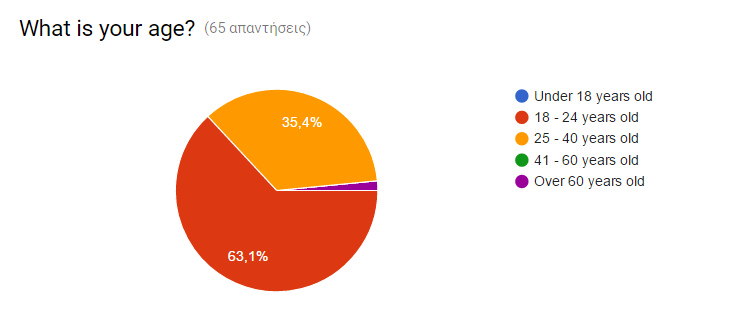
\includegraphics[width=1\columnwidth]{1}
\caption{The ages of the users that took part in our questionnaire.}
\end{figure}

\begin{figure}[H]
\centering
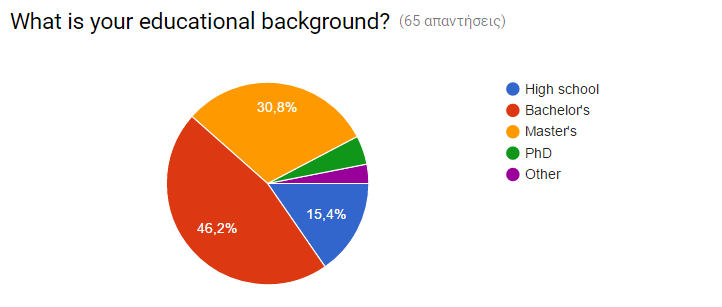
\includegraphics[width=1\columnwidth]{2}
\caption{The educational background of the users that took part in our 
questionnaire.}
\end{figure}

\begin{figure}[H]
\centering
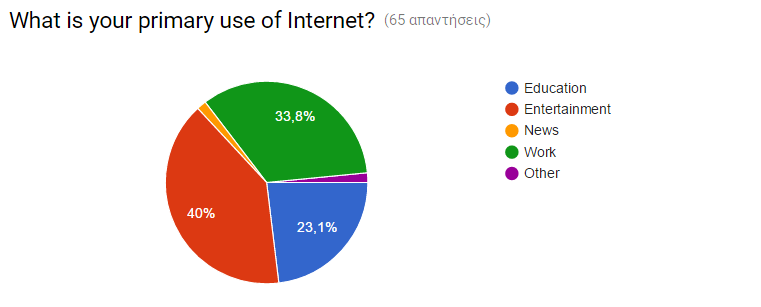
\includegraphics[width=1\columnwidth]{3}
\caption{The primary reason that the users that took part in our questionnaire 
use the Internet.}
\end{figure}

\begin{figure}[H]
\centering
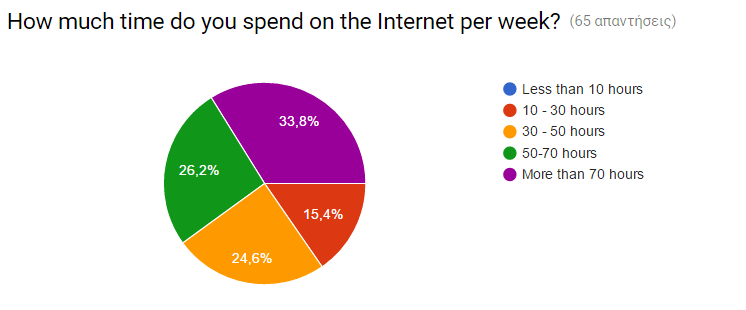
\includegraphics[width=1\columnwidth]{4}
\caption{The time of use of the Internet per week of those who took part in our 
questionnaire.}
\end{figure}

\begin{figure}[H]
\centering
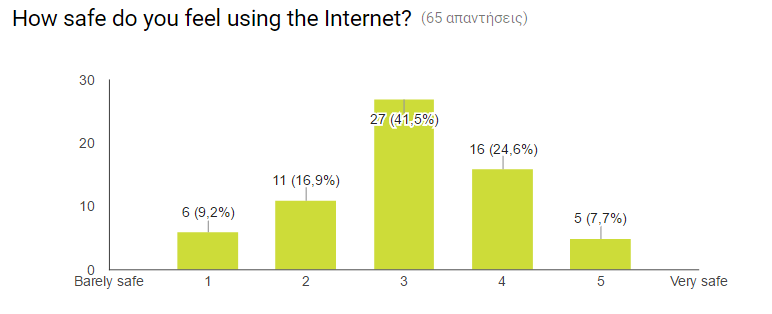
\includegraphics[width=1\columnwidth]{5}
\caption{The ranking of the users that took part in our questionnaire answering 
the question: ``How safe do you feel using the Internet?''. The rankings (1 to 5) 
are displayed in the x-axis.}
\end{figure}

Observing the diagram we noticed that most of the respondents  do not feel the 
Internet as a safe place.They might be  aware of the existence of some dangers 
on the Internet, but they are not feeling extremely threatened.

\subsubsection{Privacy}

These questions tried to find out whether the users have any awareness and care 
about their personal information protection and disclosure.

\begin{figure}[H]
\centering
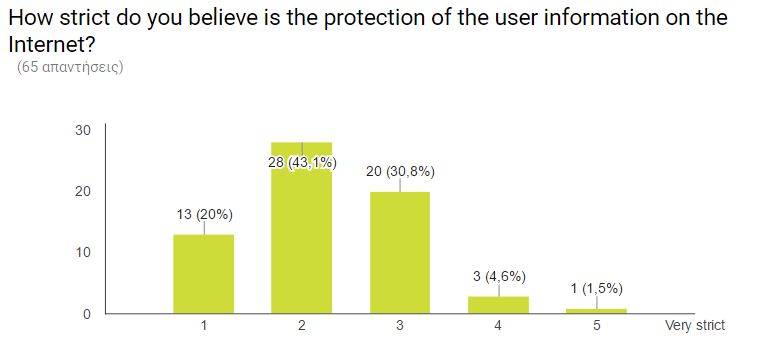
\includegraphics[width=1\columnwidth]{6}
\caption{The ranking of the users that took part in our questionnaire answering
the question: ``How strict do you believe is the protection of the user 
information on the Internet?''. The rankings (1 to 5) are displayed in the 
x-axis.}
\end{figure}

\begin{figure}[H]
\centering
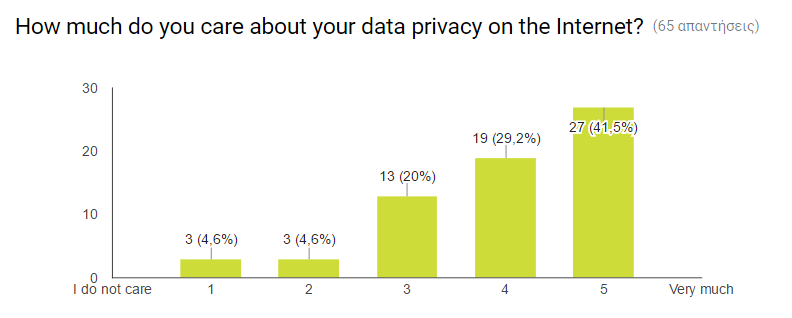
\includegraphics[width=1\columnwidth]{7}
\caption{The ranking of the users that took part in our questionnaire answering
the question: ``How much do you care about your data privacy on the Internet?''. 
The rankings (1 to 5) are displayed in the x-axis.}
\end{figure}

\begin{figure}[H]
\centering
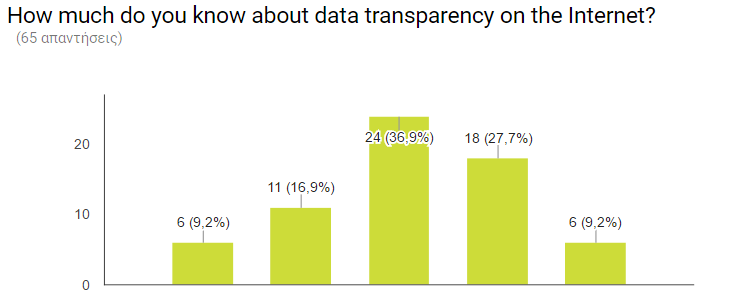
\includegraphics[width=1\columnwidth]{8}
\caption{The ranking of the users that took part in our questionnaire answering
the question: ``How much do you know about data transparency on the Internet?''. 
The rankings (1 to 5) are displayed in the x-axis.}
\end{figure}

\begin{figure}[H]
\centering
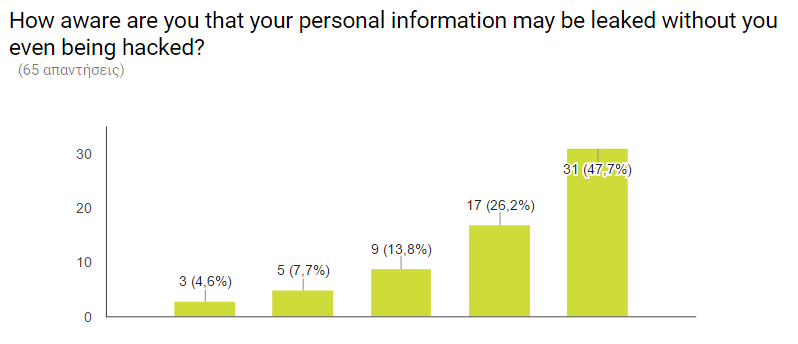
\includegraphics[width=1\columnwidth]{9}
\caption{The ranking of the users that took part in our questionnaire answering
the question: ``How aware are you that your personal information may be leaked 
without you even being hacked?''. The rankings (1 to 5) are displayed in the 
x-axis.}
\end{figure}

Most of the volunteers care about their data privacy, although they believe that 
there is not enough.

\subsubsection{Routing and data storage}

In this section, we want to find out if the users are informed at the topics of 
traffic routing and  data storage.

\begin{figure}[H]
\centering
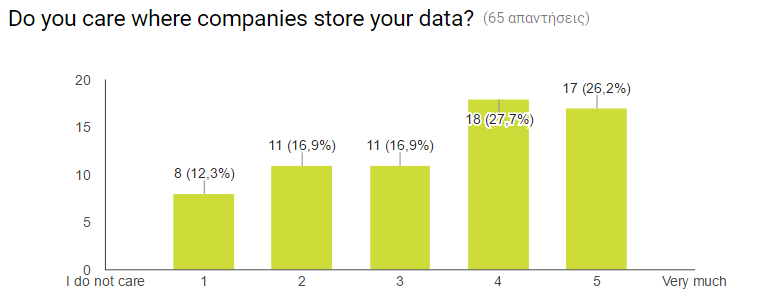
\includegraphics[width=1\columnwidth]{10}
\caption{The ranking of the users that took part in our questionnaire answering
the question: ``Do you care where companies store your data?''. The rankings (1 
to 5) are displayed in the x-axis.}
\end{figure}

\begin{figure}[H]
\centering
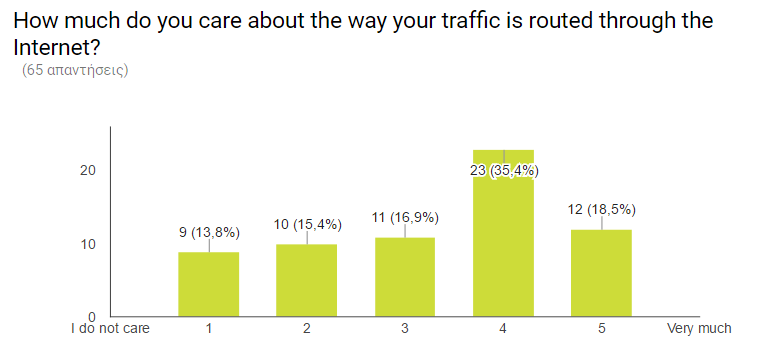
\includegraphics[width=1\columnwidth]{11}
\caption{The ranking of the users that took part in our questionnaire answering
the question: ``How much do you care about the way your traffic is routed 
through the Internet?''. The rankings (1 to 5) are displayed in the x-axis.}
\end{figure}

\begin{figure}[H]
\centering
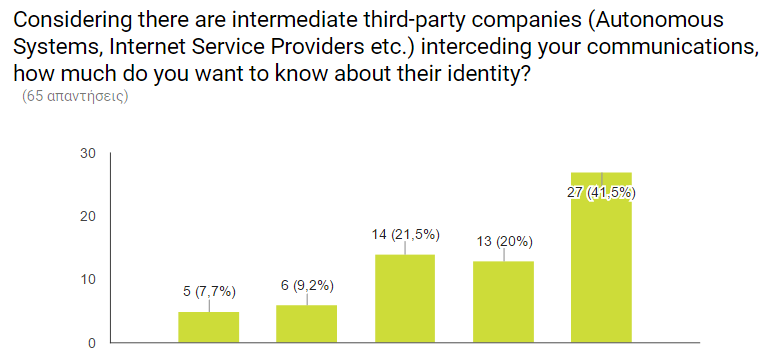
\includegraphics[width=1\columnwidth]{12}
\caption{The ranking of the users that took part in our questionnaire answering
the question: ``Considering there are intermediate third-party companies 
(Autonomous Systems, Internet Service Providers etc.) interceding your 
communications, how much do you want to know about their identity?''. The 
rankings (1 to 5) are displayed in the x-axis.}
\end{figure}

\begin{figure}[H]
\centering
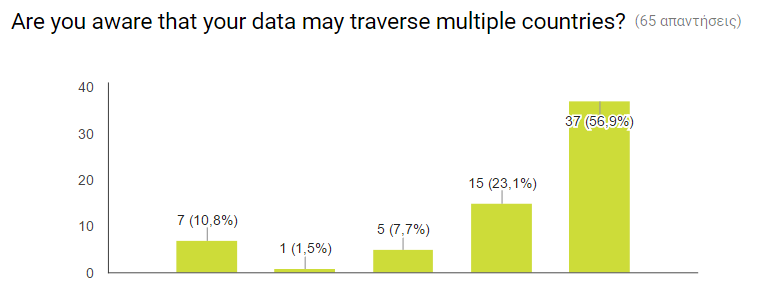
\includegraphics[width=1\columnwidth]{13}
\caption{The ranking of the users that took part in our questionnaire answering
the question: ``Are you aware that your data may traverse multiple countries?''. The
rankings (1 to 5) are displayed in the x-axis.}
\end{figure}

Most of the volunteers  seem to be concerned about their traffic routing and the 
data  storage locations, even if they are not may be fully informed or experts 
on this topic. 

\subsubsection{Law enforcement and regulations}

In this section we want to find out the extend of the knowledge of the 
respondents regarding laws and legislations of internet traffic.

\begin{figure}[H]
\centering
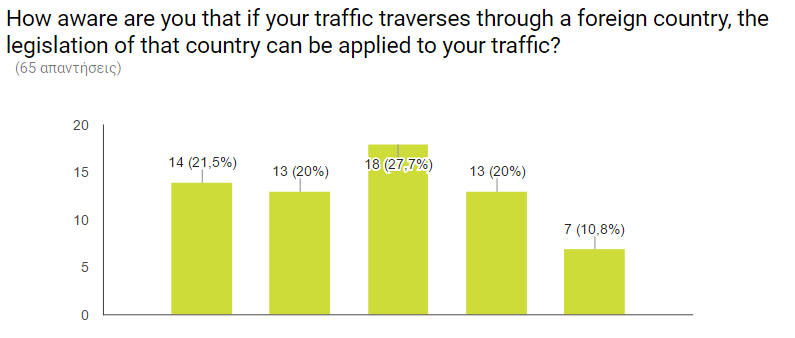
\includegraphics[width=1\columnwidth]{14}
\caption{The ranking of the users that took part in our questionnaire answering
the question: ``How aware are you that if your traffic traverses through a 
foreign country, the legislation of that country can be applied to your 
traffic''. The rankings (1 to 5) are displayed in the x-axis.}
\end{figure}

\begin{figure}[H]
\centering
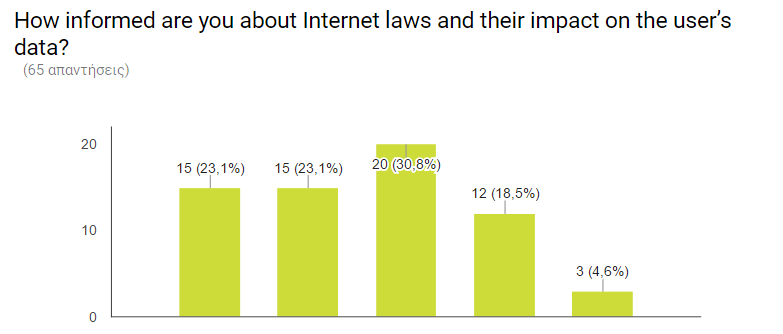
\includegraphics[width=1\columnwidth]{15}
\caption{The ranking of the users that took part in our questionnaire answering
the question: ``How informed are you about Internet laws and their impact on the 
user's data?''. The rankings (1 to 5) are displayed in the x-axis.}
\end{figure}

\begin{figure}[H]
\centering
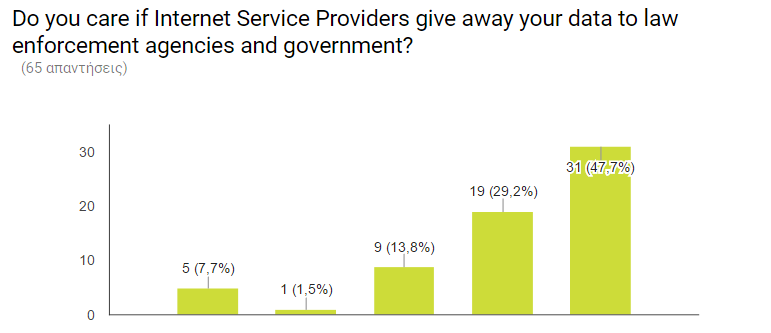
\includegraphics[width=1\columnwidth]{16}
\caption{The ranking of the users that took part in our questionnaire answering
the question: ``Do you care if Internet Service Providers give away your data to 
law enforcement agencies and government?''. The
rankings (1 to 5) are displayed in the x-axis.}
\end{figure}

\begin{figure}[H]
\centering
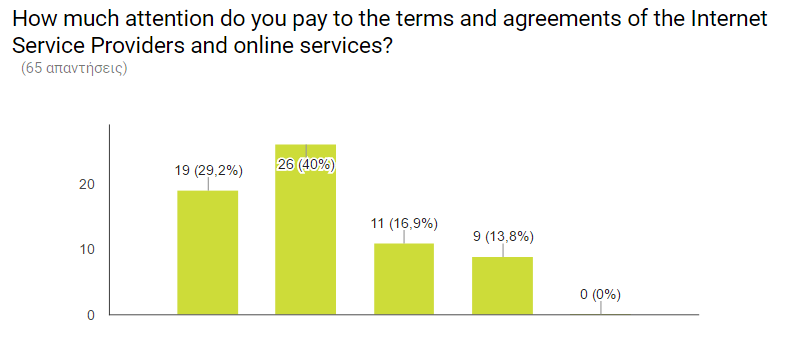
\includegraphics[width=1\columnwidth]{17}
\caption{The ranking of the users that took part in our questionnaire answering
the question: ``How much attention do you pay to the terms and agreements of the 
Internet Service Providers and online services''. The rankings (1 to 5) are 
displayed in the x-axis.}
\end{figure}

We observe that most users are not aware of the legislations regarding the 
internet traffic. They seem concerned about the data requests from government 
agencies but on the other hand respondents don't usually read the terms and 
agreements.

\subsubsection{Online economy and advertising}

This section analyzes whether the respondents are aware of the targeted ads on 
web pages and services.

\begin{figure}[H]
\centering
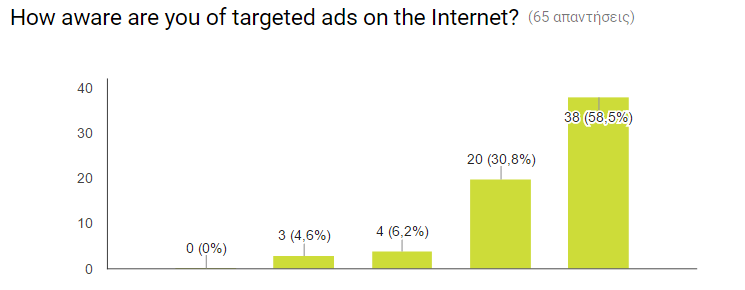
\includegraphics[width=1\columnwidth]{18}
\caption{The ranking of the users that took part in our questionnaire answering
the question: ``How aware are you of targeted ads on the Internet?''. The
rankings (1 to 5) are displayed in the x-axis.}
\end{figure}

\begin{figure}[H]
\centering
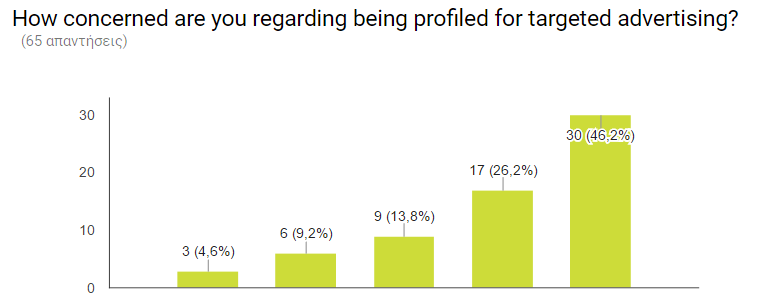
\includegraphics[width=1\columnwidth]{19}
\caption{The ranking of the users that took part in our questionnaire answering
the question: ``How concerned are you regarding being profiled for targeted 
advertising?''. The rankings (1 to 5) are displayed in the x-axis.}
\end{figure}

\begin{figure}[H]
\centering
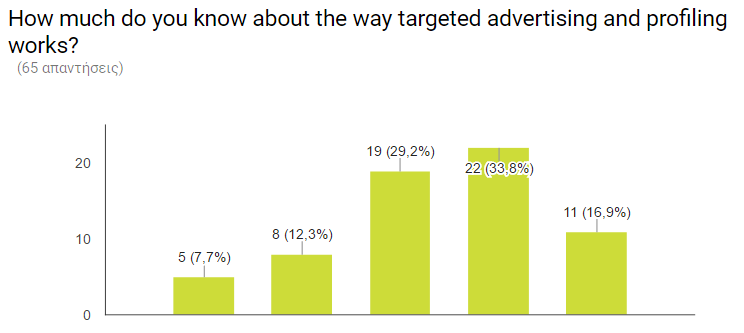
\includegraphics[width=1\columnwidth]{20}
\caption{The ranking of the users that took part in our questionnaire answering
the question: ``How much do you know about the way targeted advertising and 
profiling works?''. The rankings (1 to 5) are displayed in the x-axis.}
\end{figure}

\begin{figure}[H]
\centering
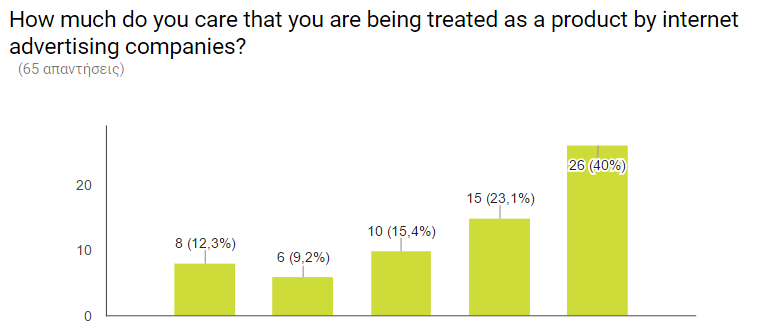
\includegraphics[width=1\columnwidth]{21}
\caption{The ranking of the users that took part in our questionnaire answering
the question: ``How much do you care that you are being treated as a product by 
internet advertising companies?''. The rankings (1 to 5) are displayed in the 
x-axis.}
\end{figure}

Most respondents are informed about targeted ads although they don't know how 
the ads works exactly.

\subsubsection{User trust}

In this section we try to understand some aspects on trust from the user's point 
of view.

\begin{figure}[H]
\centering
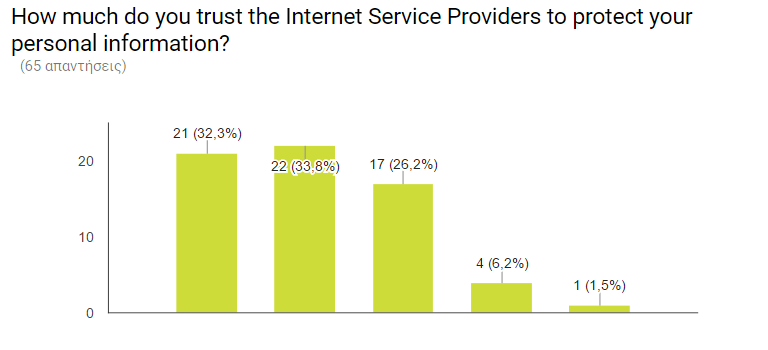
\includegraphics[width=1\columnwidth]{22}
\caption{The ranking of the users that took part in our questionnaire answering
the question: ``How much do you trust the Internet Service Providers to protect 
your personal information?''. The rankings (1 to 5) are displayed in the x-axis.}
\end{figure}

\begin{figure}[H]
\centering
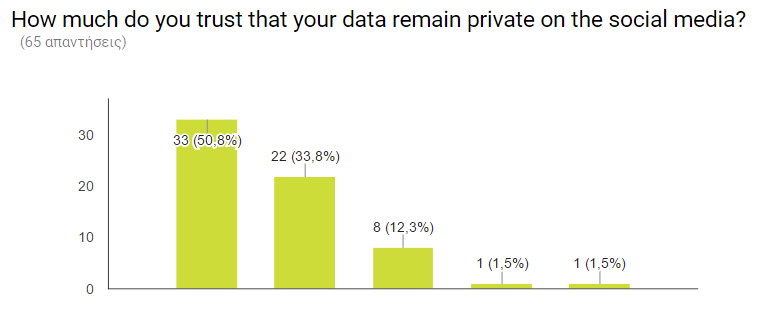
\includegraphics[width=1\columnwidth]{23}
\caption{The ranking of the users that took part in our questionnaire answering
the question: ``How much do you trust that your data remain private on the 
social media?''. The rankings (1 to 5) are displayed in the x-axis.}
\end{figure}

\begin{figure}[H]
\centering
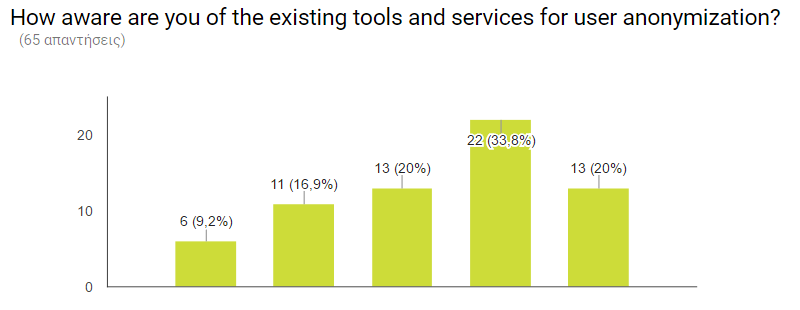
\includegraphics[width=1\columnwidth]{24}
\caption{The ranking of the users that took part in our questionnaire answering
the question: ``How aware are you of the existing tools and services for user 
anonymization?''. The rankings (1 to 5) are displayed in the x-axis.}
\end{figure}

\begin{figure}[H]
\centering
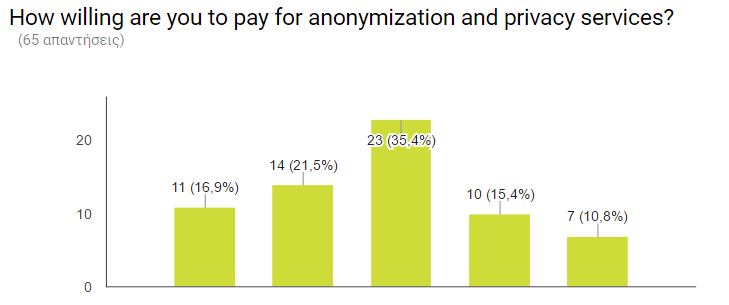
\includegraphics[width=1\columnwidth]{25}
\caption{The ranking of the users that took part in our questionnaire answering
the question: ``How willing are you to pay for anonymization and privacy 
services?''. The rankings (1 to 5) are displayed in the x-axis.}
\end{figure}

\subsubsection{Potential outcome}

With the following question we tried to understand whether our questionnaire on 
the online data transparency managed to make the users more concerned.  

\begin{figure}[H]
\centering
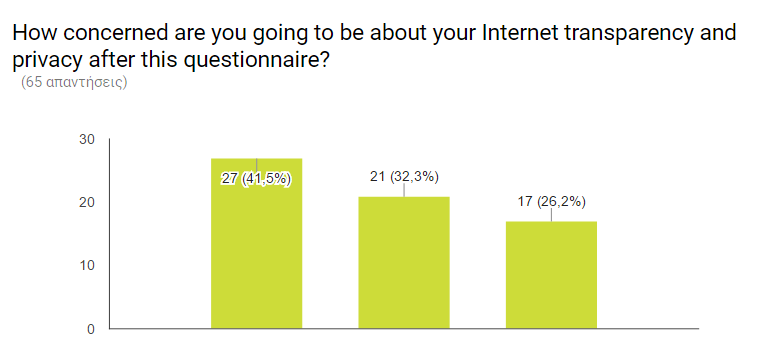
\includegraphics[width=1\columnwidth]{26}
\caption{The ranking of the users that took part in our questionnaire answering
the question: ``How concerned are you going to be about your Internet 
transparency and privacy after this questionnaire?''. The
rankings (1 to 3) are displayed in the x-axis, where 1 represents the value 
``The same'' and 3 represents the value ``Much more concerned''.}
\end{figure}



	\bibliographystyle{abbrv}
	\bibliography{references}

\end{document}
